%! Author = hp

% Preamble
\documentclass[11pt]{article}

% Packages
\usepackage{amsthm}
\usepackage[utf8]{inputenc}
\usepackage[T1]{fontenc}
\usepackage{blindtext}
\usepackage[a4paper, margin=2cm, includefoot, heightrounded]{geometry}
\usepackage{csquotes}
\usepackage{titlesec}
\usepackage{sectsty}
\usepackage{amsmath}
\usepackage[english]{babel}
\usepackage{pxfonts}
\usepackage{enumitem}
\usepackage{mathtools}
\usepackage{amssymb}
\usepackage{biblatex}
\usepackage{fancyhdr}
\usepackage[charter]{mathdesign}
\usepackage{xcolor}
\usepackage{amsfonts}
\usepackage{algorithm}
\usepackage{algpseudocode}
\usepackage{algorithmicx}
\usepackage{bm}
\usepackage{graphicx}
\usepackage{caption}
\usepackage{subcaption}
\usepackage{hyperref}


\pagestyle{fancy}
\fancyhf{}
\fancyhead[LE,RO]{
    Fistname Sirname\\
    Matr. Nr.: 123456\\
    Datum: Date
}
\fancyhead[RE,LO]{
    \textbf{University} \\
    Tätigkeitsbericht zu Robotik-Anwendungen\\
    Wintersemester 2021/2022
}
\fancyfoot[LE,RO]{\thepage}

\renewcommand{\headrulewidth}{1pt}
\renewcommand{\footrulewidth}{1pt}

\graphicspath{{../}}
\hypersetup {
    colorlinks=true,
    linkcolor=blue,
    urlcolor=blue
}


% Document
\begin{document}
 \mbox{}
    \section*{\centering{Drink filling level and foam-drink ratio measurements}}
    With the coming cold of the winter season, comes the winter semester, hence as usual the course Robotik-Anwendungen.
    This year's project \enquote{Babo-Bartender Robot} consisted in the development of a robot system to automatic
    serve drinks.
    The robot should be capable of either serving drinks taken from a defined position and opened, or tapping drinks from
    a defined position.
    With a virtual budget of 750 Euro, 1) the kinematics and dynamics of the system were to be simulated with the appropiate
    actors and 2) the filling level of the glass and the ratio foam-drink were to be continuously measured.
 
    Due to the fact that robots that dispense food and drinks existed since the dawn of time, i have decided to undertake
    the second task, of which this report will present the result.

    \paragraph*{}
    To solve the above-mentioned task, multiple ideas were collected and analysed.
    The required features, in order of priority are as follows: the system needed to be affordable, reliable (repeatable
    and reproducible measurements), hygienic and sanitary, quick, scalable (easily repairable, extensible, low-dependencies).

    Possible methods for level measurement could be achieved by using 1) \textbf{Laser transceivers}, values recorded by
    the laser sensors would correspond to different region of the glass filling state, 2) \textbf{Ultrasonic sensors} which
    would measure the distance to the uppermost part of the content of the drink, 3) \textbf{weight sensors} with which
    the height of the drink could be approximated using its weight, 4) \textbf{Capacitive sensors}, which when placed
    at certain positions of the glass would indicate if the content of the glass was reached and 5) \textbf{camera} to
    differentiate the levels using image processing technics.

    By process of elimination, the camera proved to be the idea sensor for our task.
    This is due to the fact that (1), (4) could only support a finite amount of sensors, of readings and hence won't
    provide accurate continuous measurement.
    (1), (3), (4) are all glass dependent and (2) is unpredictable as unexpected reflections, absorptions of ultrasonic
    waves at the surface of the liquid could occur.
    Moreover, apart from (5), none could provide the accurate ration between drink and foam.
    There are no free lunch!
    Despite its advantages compared to the other alternatives, the accuracy and performance of the camera depend on the
    programming.

    \paragraph*{}
    How does one detect the level of drink and foam in a glass?
    Using Image processing: In the digital image processing, an image is \textit{width} x \textit{height} tensor
    \footnote{here as multidimensional array} usually comprised of three levels (r,g,b).
    With the help of matrix manipulation technics, images can be sharpened, blurred, rotated, edges can be found, \ldots .
    To process images, libraries are usually used not only to save time, but because of their efficiency as images can
    be processed in a parallel fashion on the CPU or GPU.
    A popular and free programming library to process images is OpenCV.
    Officially launched by Intel in 1999, it is the De facto library for image processing.
    OpenCV is written in C++ but provides bindings for Java and Python.

    Extracting the needed information from the images proved to be very difficult: A glass is transparent, reflective,
    refractive.
    The \textbf{canny} edge detection algorithm after an \textbf{adaptive threshold} doesn't provide the
    contour of the glass due to the fact that the edges of the glass are transparent.

    After multiple failed attempts, the successful implementation consisted of two phases:
    \begin{enumerate}
       \item the empty glass to be filled was to be extracted from the background.
    For this purpose, an image without the glass is taken as well as another containing it.
    Both images are first smoothed with \textbf{Gaussian blur}\footnote{\href{https://aryamansharda.medium.com/image-filters-gaussian-blur-eb36db6781b1}{Gaussian blur}} to remove unwanted noise, then sharpened with a
    sharpening algorithm i.e. \textbf{unsharp masking}\footnote{\href{https://www.cambridgeincolour.com/tutorials/unsharp-mask.htm}{Unsharp mask}} to highlight the edges of the glass.
    The difference of both image is made to extract the empty glass.
    The glass is then removed by applying the \textbf{canny}\footnote{\href{https://justin-liang.com/tutorials/canny/}{canny}} edge detection algorithm to an \textbf{adaptive threshold}\footnote{\href{https://homepages.inf.ed.ac.uk/rbf/HIPR2/adpthrsh.htm}{Adaptive threshold}}-ed
       image and selecting the contour with the largest area.
       \item then as the glass is getting filled, the different areas of the liquid are extracted by color specified in
    a range of values.
    Foam is usually white and would correspond to the HSV range (0,48,148)-(179,255,255) while the drink, in the case
    of beer can be bounded by (0,133,0) and (12,255,135).
    \end{enumerate}
    (1) provides a contour around the glass and (2) a contour around the foam and around the drink.
    The computation of the ratios can be achieved either by using the area of the contours with \textbf{cv2.contourArea}
    or with the height of bounding boxes around each contour.
    With the latter, the ratio of foam and drink in the glass results from the division of the height of the corresponding
    bounding box with that of the glass.
    This method outputs the ratio of foam and drink as percentage of the complete glass.
    The filling level results from the summation of both of these ratios.

    \fancyhead{}
    \renewcommand{\headrulewidth}{0pt}

    \begin{figure}
        \centering
        \begin{subfigure}[b]{0.2\textwidth}
            \centering
            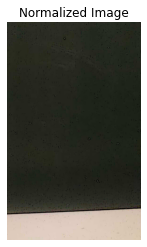
\includegraphics[scale=0.7]{empty_image}
            \caption{Glassless image}
        \end{subfigure}
        \begin{subfigure}[b]{0.2\textwidth}
            \centering
            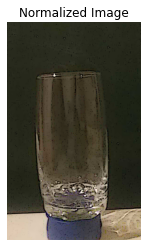
\includegraphics[scale=0.7]{glass_image}
            \caption{Glass Image}
        \end{subfigure}
        \begin{subfigure}[b]{0.2\textwidth}
            \centering
            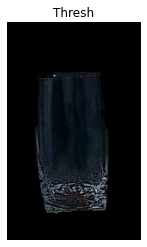
\includegraphics[scale=0.7]{glass_extraction}
            \caption{Glass extraction}
        \end{subfigure}
        \begin{subfigure}[b]{0.2\textwidth}
            \centering
            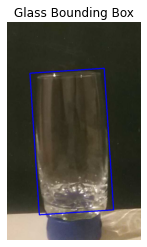
\includegraphics[scale=0.7]{glass_box}
            \caption{Bounding box}
        \end{subfigure}
        \caption{Empty glass extraction}
        \label{fig:figure}
    \end{figure}

    \begin{figure}
        \centering
        \begin{subfigure}[b]{0.2\textwidth}
            \centering
            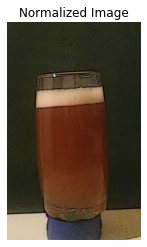
\includegraphics[scale=0.7]{glass_filling}
            \caption{Glassless image}
        \end{subfigure}
        \begin{subfigure}[b]{0.2\textwidth}
            \centering
            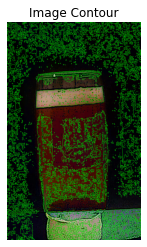
\includegraphics[scale=0.7]{contour_extraction}
            \caption{Glass Image}
        \end{subfigure}
        \begin{subfigure}[b]{0.2\textwidth}
            \centering
            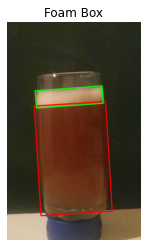
\includegraphics[scale=0.7]{beer_and_foam_boxes}
            \caption{Glass extraction}
        \end{subfigure}
        \begin{subfigure}[b]{0.2\textwidth}
            \centering
            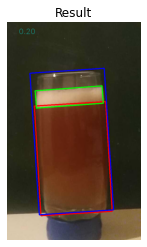
\includegraphics[scale=0.7]{output}
            \caption{Bounding box}
        \end{subfigure}
        \caption{Drink and foam extraction}
        \label{fig:figure2}
    \end{figure}

   \paragraph*{}
   This approach has multiple advantages: It works for a wide variety of glasses, of drinks with or without foam, for
   glasses in any rotation.
   Moreover, no dependencies or special requirement on the hardware is needed.
   Image processing is however in general environment dependent, i.e. a drastic change in ambient light could change the
   appearance of the foam or rather of the drink.
   This would lead to an algorithmic failure.
   To avoid as many perturbations as possible, measures have been taken.
   For example, a black background is installed behind the glass to not only avoid inconsistencies in the images, but also
   to absorb colors created by the refraction and refection of light by the glass.
   Another problem related to image processing, is the fact that image processing is a resource demanding process and
   requires a powerful computing unit.

   \paragraph*{}
    Our bartending robot needs to be intelligent!
    For the processing unit, we decided to opt for a 1GiB version Raspberry PI 4, as it offers enough power for the image
    processing task, is programmable in Python, a simple programming language and supports hardware-level multitasking
    (processes, threads, SIMD) with which the different components of the robots could work and communicate in
    parallel.
    Furthermore, it can power two external display systems, from which customers can place others and receive notifications.
    With an internet connection, the Raspberry PI can be remotely accessed and programmed.
    This allows for further development and repairs without the need for physically displacement of the processing unit.

    \paragraph*{}
    The camera of choice is the Raspberry PI camera v2.1, as it provides a simple interface to communicate with a
    Raspberry PI.

    \begin{figure}
        \centering
        \begin{subfigure}[b]{0.4\textwidth}
            \centering
            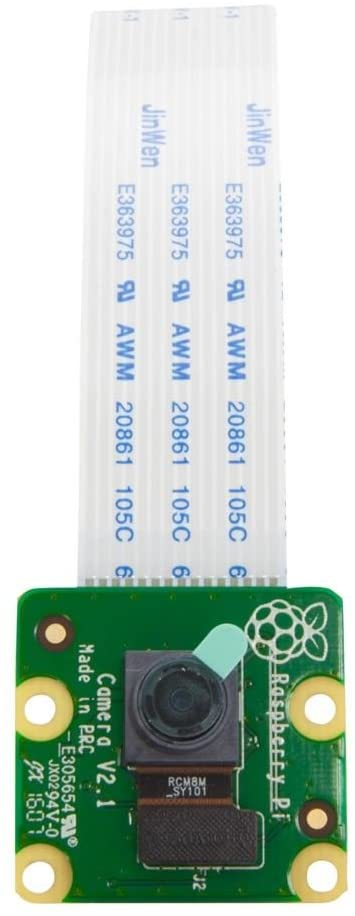
\includegraphics[scale=0.2]{51fSegjSN+L._AC_SL1000_}
            \caption{Raspberry PI Camera v2.1}
        \end{subfigure}
        \begin{subfigure}[b]{0.4\textwidth}
            \centering
            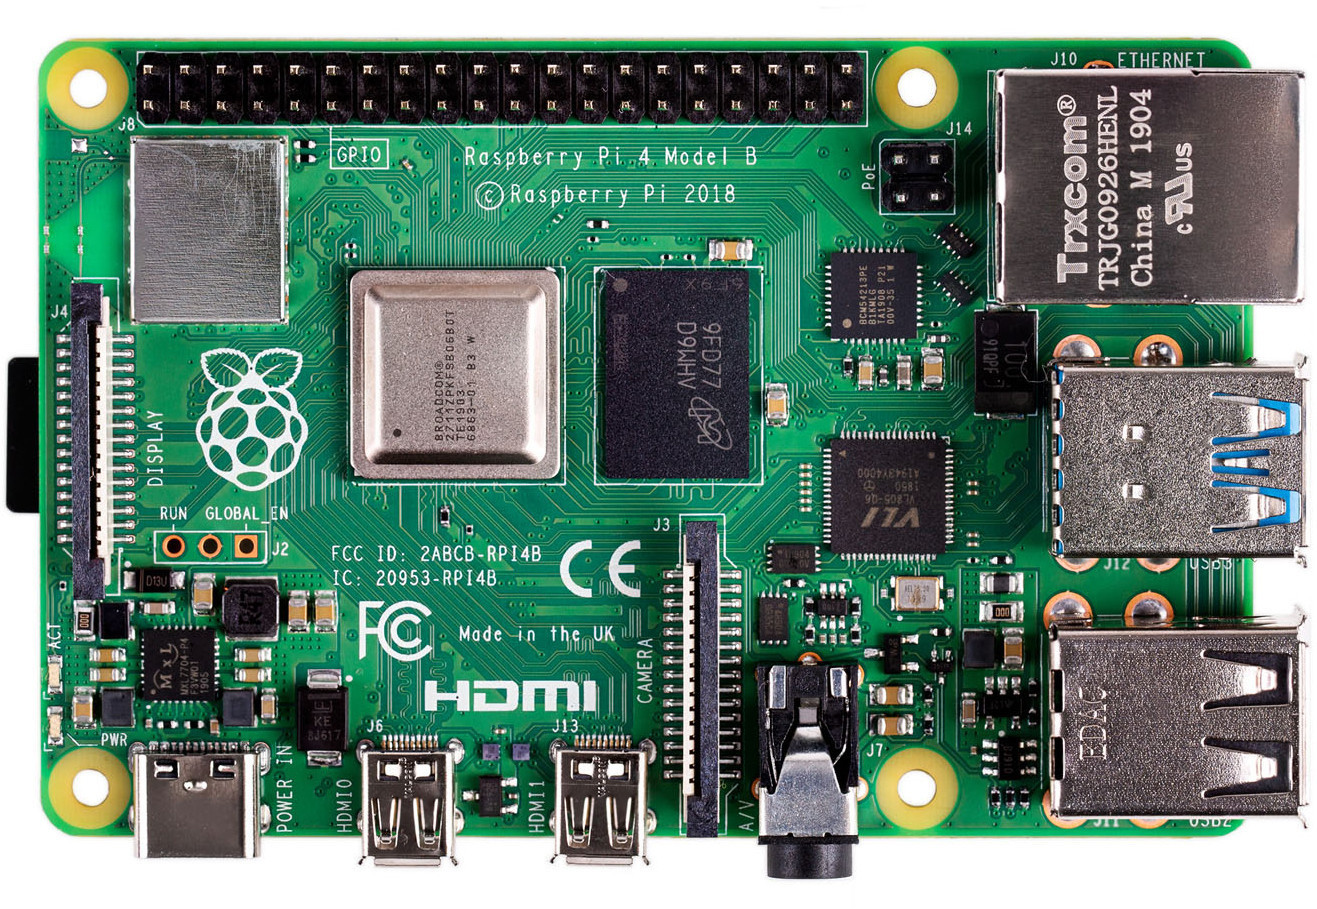
\includegraphics[scale=0.1]{raspberry-pi-4-model-b}
            \caption{Raspberry PI 4}
        \end{subfigure}
        \caption{Sensor and processing Unit}
        \label{fig:figure3}
    \end{figure}

    \paragraph*{}
    The total cost of the sensor amount to around 75 Euro: 45 Euro for the Raspberry PI and 30 for the camera.
    This cost can be reduced by choosing alternative and more affordable cameras like the Arducam 5MP for 10 Euro or an older
    version of a Raspberry PI.

\end{document}
